\documentclass[landscape, 11pt]{report}

% Packages
\usepackage[landscape]{geometry}
\usepackage{amsmath}
\usepackage{xcolor}
\usepackage[utf8]{inputenc}
\usepackage[russian]{babel}
\usepackage{geometry}
\usepackage{graphicx}

% Options
\graphicspath{ {../figures/} {./figures/}}
\geometry{left=2.5cm,right=2.5cm,top=2.5cm,bottom=2.5cm}
\setlength\parindent{0pt}

% Title
\title{
	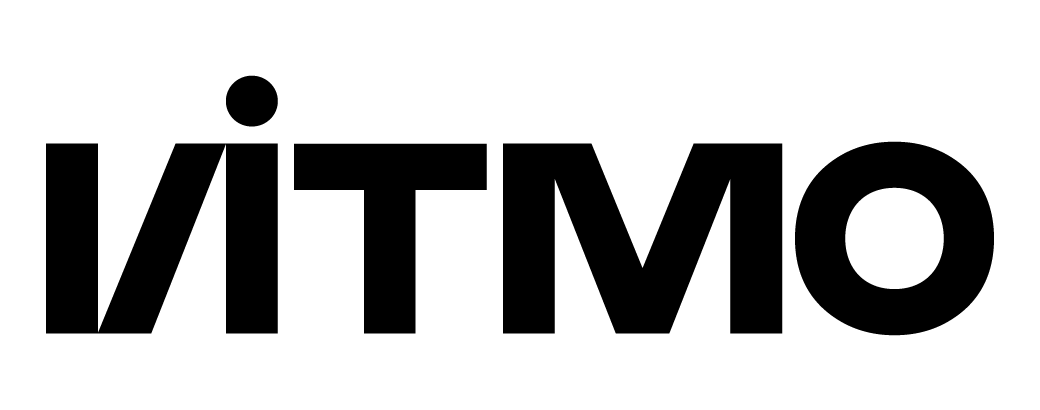
\includegraphics[scale=0.07]{logo}\\
	\vspace{0.5em}
	Языки программирования. Семантика и система типов\\
	\vspace{0.2em}
	\Large Теоретическое задание. Тема 3
}
\author{Бронников Егор}
\date{}


\begin{document}
	
	% Титул
	
	\maketitle
	
	\vspace{-0.5cm}
	\hrule
	\vspace{0.5cm}
	
	% Задание 1
	
	\textbf{Задание 1.} $(\lambda f . \, (f \, \{ \text{\color{purple}succ} \, \text{\color{blue}0}, \, \text{\color{purple}iszero} \, (f \, \{\text{\color{blue}0}, \, \text{\color{purple}false}\}).a \}).b) \, (\lambda t . \, \{a = t.1, \, b = t.2\})$
	
	\vspace{0.2cm}
	
	\textit{1. Дополнение пропущенных аннотаций.}
	
	$(\lambda f : \boldsymbol{\{a: Nat, \, b: Bool\}}. \, (f \, \{ \text{\color{purple}succ} \, \text{\color{blue}0}, \, \text{\color{purple}iszero} \, (f \, \{\text{\color{blue}0}, \, \text{\color{purple}false}\}).a \}).b) \, (\lambda t : \boldsymbol{Nat \times Bool}. \, \{a = t.1, \, b = t.2\})$
	
	\vspace{0.2cm}
	
	\textit{2. Дерево вывода типа.}
	
	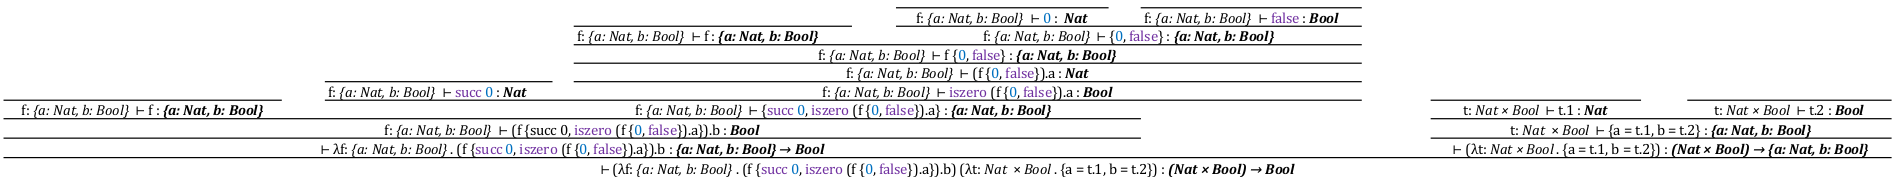
\includegraphics[scale=0.35]{task-1.png}

	\vspace{0.3cm}

	\small \textit{Примечание.} Рекомендуется изучить исходный Excel-документ \verb|source.xlsx|. \normalsize

	\vspace{0.2cm}
	\hrule
	\vspace{0.5cm}	
	
	% Задание 2
	
	\textbf{Задание 2.}

	\vspace{0.2cm}

	\textit{Условие.} В нетипизированном $\lambda$-исчисления, пары термов могут быть представлены при помощи кодировки Чёрча. Можно ли использовать это представление, чтобы представить пары как производную форму поверх простого типизированного $\lambda$-исчисления с логическими и арифметическими выражениями?

	\vspace{0.2cm}

	\textit{Ответ.} Да, можно.
	
	Для начала стоит напомнить определение пары в кодировке Чёрча в нетипизированном $\lambda$-исчислении:
	
	\begin{center}
		$pair := \lambda x . \, \lambda y. \, \lambda z. \, z \, x \, y$\\
		$first := \lambda p . \, p \, (\lambda x . \, \lambda y . \, x)$\\
		$second := \lambda p . \, p \, (\lambda x . \, \lambda y . \, y)$
	\end{center}
	
	Теперь перейдём к описанию определение пары в кодировке Чёрча в простом типизированном $\lambda$-исчислении:

	\begin{center}
		$pair := \lambda x : T_1. \, \lambda y : T_2. \, \lambda z : (T_1 \rightarrow T_2 \rightarrow T) \, . \, z \, x \, y$\\
		$first := \lambda p : (T_1 \times T_2) \, . \, p \, (\lambda x : T_1 \, . \, \lambda y : T_2 \, . \, x)$\\
		$second := \lambda p : (T_1 \times T_2) \, . \, p \, (\lambda x : T_1 \, . \, \lambda y : T_2 \, . \, y)$\\
		$(T_1 \times T_2) := (T_1 \rightarrow T_2 \rightarrow T \rightarrow T)$
	\end{center}

	\newpage

	\textit{a. Функция раскрытия сокращения.}
	
	\begin{itemize}
		\item {\textit{Пара}

		$e(pair) = e(\lambda x : T_1. \, \lambda y. : T_2 \, \lambda z : (T_1 \rightarrow T_2 \rightarrow T) \, . \, z \, x \, y) = \lambda x : T_1. \, \lambda y : T_2. \, \lambda z : (T_1 \rightarrow T_2 \rightarrow T) \, . \, e(z) \, e(x) \, e(y)$
		}

		\item {\textit{Проекции}
	
		$e(first) = e(\lambda p : (T_1 \times T_2) \, . \, p \, (\lambda x : T_1 \, . \, \lambda y : T_2 \, . \, x)) = \lambda p : (T_1 \times T_2) \, . \, p \, (\lambda x : T_1 \, . \, \lambda y : T_2 \, . \, e (x))$\\
		$e(second) := e(\lambda p : (T_1 \times T_2) \, . \, p \, (\lambda x : T_1 \, . \, \lambda y : T_2 \, . \, y)) = \lambda p : (T_1 \times T_2) \, . \, p \, (\lambda x : T_1 \, . \, \lambda y : T_2 \, . \, e(y))$
		}
	
		\item {\textit{Тип-произведения}

		$e(T_1 \times T_2) = e(T_1 \rightarrow T_2 \rightarrow T \rightarrow T) = e(T_1) \rightarrow e(T_2) \rightarrow e(T) \rightarrow e(T)$\\
		}
		
	\end{itemize}

	\textit{b. Сохранение вычисления и типизации}

	\begin{itemize}
	\item \textit{Сохранение вычисления:} Да, функция раскрытия сокращений сохраняет вычисление, поскольку просто переводит выражения из одного представления в другое, не меняя семантику.
	
	\item \textit{Сохранение типизации:} Да, сохраняется. Каждое выражение в новом представлении имеет тип, который зависит от типов $first$ и $second$, а также типов проекций, что отражается в определении новых функций.
	\end{itemize}

	\hspace{0.8cm} Таким образом, функция раскрытия сокращений сохраняет и вычисление, и типизацию. Если бы это не работало, это могло бы быть из-за несоответствия типов или неправильной интерпретации функций проекции. Например, если бы мы неправильно определили тип $T_1 \times T_2$ или проекции $first$ и $second$, это могло бы привести к нарушению типизации.
\end{document}
